\documentclass[14pt]{extbook}
\usepackage{multicol, enumerate, enumitem, hyperref, color, soul, setspace, parskip, fancyhdr} %General Packages
\usepackage{amssymb, amsthm, amsmath, latexsym, units, mathtools} %Math Packages
\everymath{\displaystyle} %All math in Display Style
% Packages with additional options
\usepackage[headsep=0.5cm,headheight=12pt, left=1 in,right= 1 in,top= 1 in,bottom= 1 in]{geometry}
\usepackage[usenames,dvipsnames]{xcolor}
\usepackage{dashrule}  % Package to use the command below to create lines between items
\newcommand{\litem}[1]{\item#1\hspace*{-1cm}\rule{\textwidth}{0.4pt}}
\pagestyle{fancy}
\lhead{Progress Quiz 7}
\chead{}
\rhead{Version C}
\lfoot{4173-5738}
\cfoot{}
\rfoot{Spring 2021}
\begin{document}

\begin{enumerate}
\litem{
Solve the quadratic equation below. Then, choose the intervals that the solutions $x_1$ and $x_2$ belong to, with $x_1 \leq x_2$.\[ 20x^{2} +9 x -81 = 0 \]\begin{enumerate}[label=\Alph*.]
\item \( x_1 \in [-9.31, -8.7] \text{ and } x_2 \in [0.32, 0.58] \)
\item \( x_1 \in [-1.1, -0.09] \text{ and } x_2 \in [5.3, 5.46] \)
\item \( x_1 \in [-7.67, -5.75] \text{ and } x_2 \in [0.56, 0.77] \)
\item \( x_1 \in [-46.1, -43.83] \text{ and } x_2 \in [35.99, 36.15] \)
\item \( x_1 \in [-3.85, -1.39] \text{ and } x_2 \in [1.74, 1.94] \)

\end{enumerate} }
\litem{
Graph the equation below.\[ f(x) = -(x-2)^2 - 17 \]\begin{enumerate}[label=\Alph*.]
\begin{multicols}{2}\item 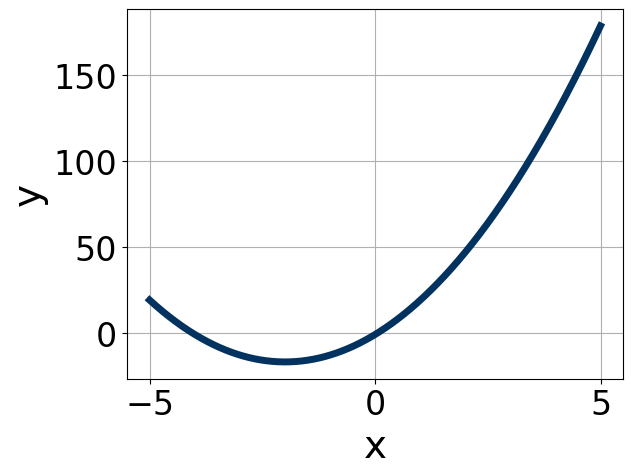
\includegraphics[width = 0.3\textwidth]{../Figures/quadraticEquationToGraphCopyAC.png}\item 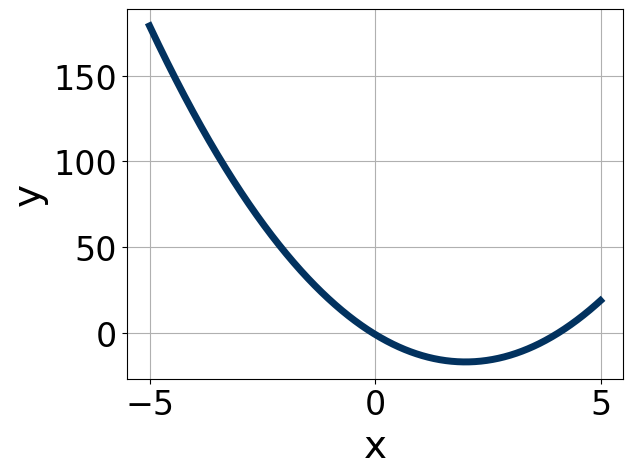
\includegraphics[width = 0.3\textwidth]{../Figures/quadraticEquationToGraphCopyBC.png}\item 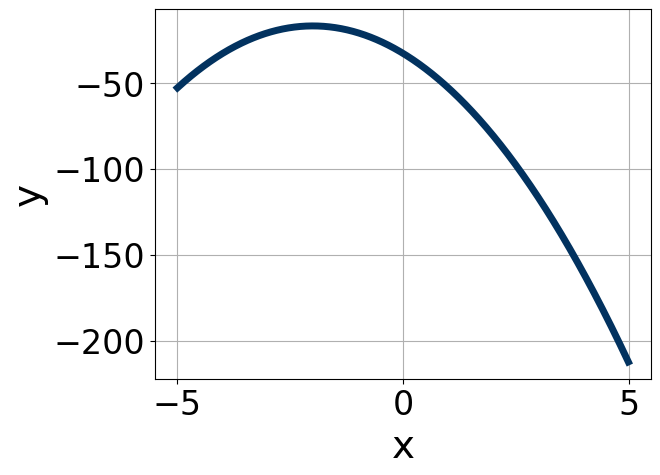
\includegraphics[width = 0.3\textwidth]{../Figures/quadraticEquationToGraphCopyCC.png}\item 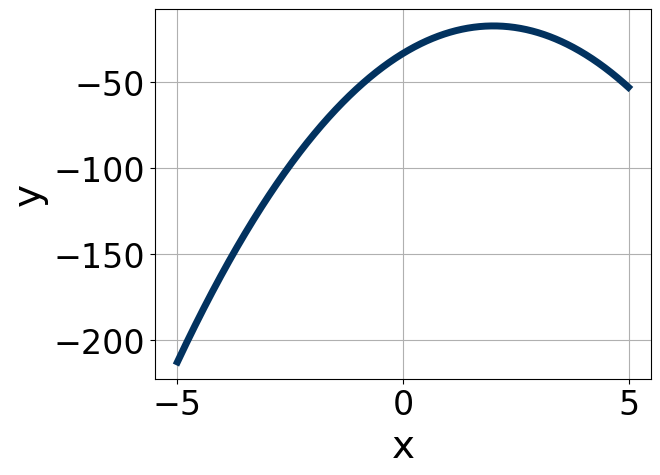
\includegraphics[width = 0.3\textwidth]{../Figures/quadraticEquationToGraphCopyDC.png}\end{multicols}\item None of the above.
\end{enumerate} }
\litem{
Solve the quadratic equation below. Then, choose the intervals that the solutions belong to, with $x_1 \leq x_2$ (if they exist).\[ 16x^{2} +11 x -7 = 0 \]\begin{enumerate}[label=\Alph*.]
\item \( x_1 \in [-17.5, -16.8] \text{ and } x_2 \in [5.42, 6.53] \)
\item \( x_1 \in [-1.7, -0.6] \text{ and } x_2 \in [0.14, 0.79] \)
\item \( x_1 \in [-0.9, -0.1] \text{ and } x_2 \in [0.97, 2] \)
\item \( x_1 \in [-24.3, -22.7] \text{ and } x_2 \in [22.9, 24.15] \)
\item \( \text{There are no Real solutions.} \)

\end{enumerate} }
\litem{
Solve the quadratic equation below. Then, choose the intervals that the solutions $x_1$ and $x_2$ belong to, with $x_1 \leq x_2$.\[ 10x^{2} -37 x -36 = 0 \]\begin{enumerate}[label=\Alph*.]
\item \( x_1 \in [-8.86, -6.91] \text{ and } x_2 \in [42.81, 45.66] \)
\item \( x_1 \in [-4.28, -2.26] \text{ and } x_2 \in [-0.28, 0.96] \)
\item \( x_1 \in [-2.05, -1.05] \text{ and } x_2 \in [1.01, 3.85] \)
\item \( x_1 \in [-1.59, -0.74] \text{ and } x_2 \in [3.78, 5.11] \)
\item \( x_1 \in [-0.63, 0.56] \text{ and } x_2 \in [12.65, 14.01] \)

\end{enumerate} }
\litem{
Graph the equation below.\[ f(x) = -(x+4)^2 - 18 \]\begin{enumerate}[label=\Alph*.]
\begin{multicols}{2}\item 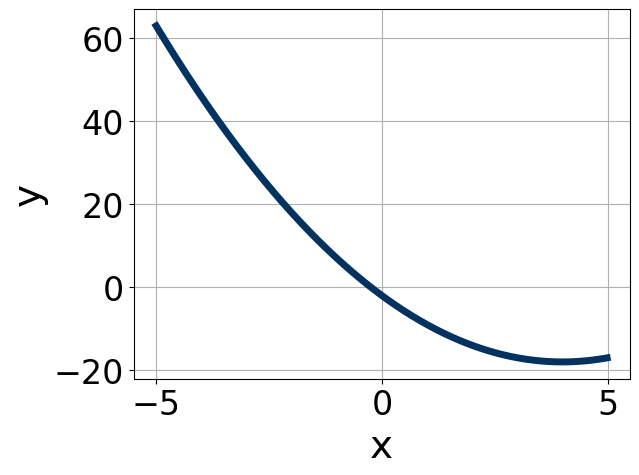
\includegraphics[width = 0.3\textwidth]{../Figures/quadraticEquationToGraphAC.png}\item 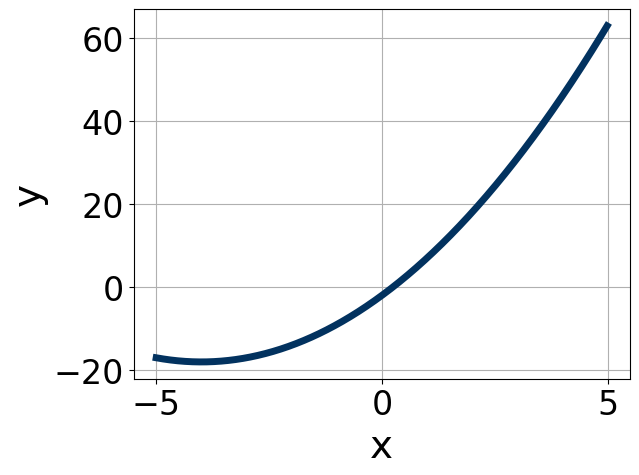
\includegraphics[width = 0.3\textwidth]{../Figures/quadraticEquationToGraphBC.png}\item 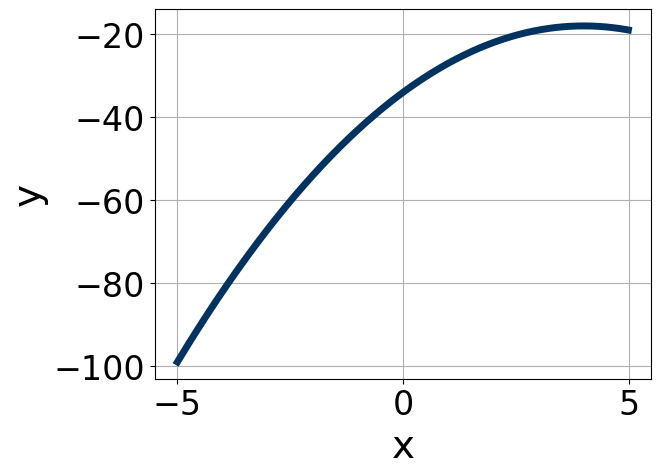
\includegraphics[width = 0.3\textwidth]{../Figures/quadraticEquationToGraphCC.png}\item 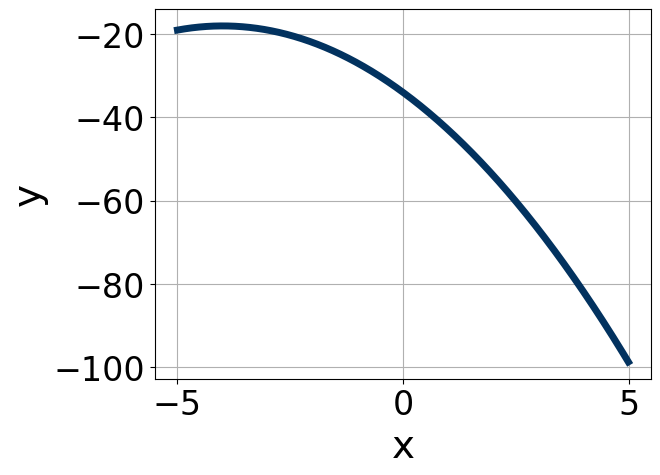
\includegraphics[width = 0.3\textwidth]{../Figures/quadraticEquationToGraphDC.png}\end{multicols}\item None of the above.
\end{enumerate} }
\litem{
Write the equation of the graph presented below in the form $f(x)=ax^2+bx+c$, assuming  $a=1$ or $a=-1$. Then, choose the intervals that $a, b,$ and $c$ belong to.
\begin{center}
    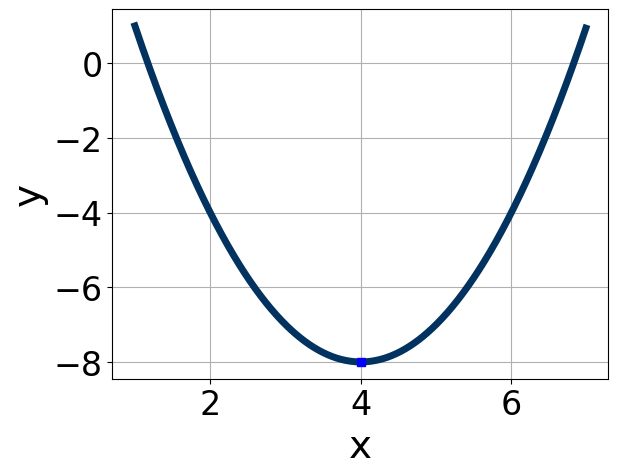
\includegraphics[width=0.5\textwidth]{../Figures/quadraticGraphToEquationC.png}
\end{center}
\begin{enumerate}[label=\Alph*.]
\item \( a \in [1, 4], \hspace*{5mm} b \in [-11, -3], \text{ and } \hspace*{5mm} c \in [8, 11] \)
\item \( a \in [1, 4], \hspace*{5mm} b \in [8, 13], \text{ and } \hspace*{5mm} c \in [8, 11] \)
\item \( a \in [1, 4], \hspace*{5mm} b \in [8, 13], \text{ and } \hspace*{5mm} c \in [22, 25] \)
\item \( a \in [-3, 0], \hspace*{5mm} b \in [-11, -3], \text{ and } \hspace*{5mm} c \in [-24, -22] \)
\item \( a \in [-3, 0], \hspace*{5mm} b \in [8, 13], \text{ and } \hspace*{5mm} c \in [-24, -22] \)

\end{enumerate} }
\litem{
Factor the quadratic below. Then, choose the intervals that contain the constants in the form $(ax+b)(cx+d); b \leq d.$\[ 24x^{2} +2 x -15 \]\begin{enumerate}[label=\Alph*.]
\item \( a \in [-0.44, 1.63], \hspace*{5mm} b \in [-19, -16], \hspace*{5mm} c \in [0.5, 1.7], \text{ and } \hspace*{5mm} d \in [18, 25] \)
\item \( a \in [10.54, 12.38], \hspace*{5mm} b \in [-6, -2], \hspace*{5mm} c \in [1.1, 2.8], \text{ and } \hspace*{5mm} d \in [2, 11] \)
\item \( a \in [1.9, 2.97], \hspace*{5mm} b \in [-6, -2], \hspace*{5mm} c \in [11.4, 13.3], \text{ and } \hspace*{5mm} d \in [2, 11] \)
\item \( a \in [3.31, 4.11], \hspace*{5mm} b \in [-6, -2], \hspace*{5mm} c \in [5.9, 6.7], \text{ and } \hspace*{5mm} d \in [2, 11] \)
\item \( \text{None of the above.} \)

\end{enumerate} }
\litem{
Factor the quadratic below. Then, choose the intervals that contain the constants in the form $(ax+b)(cx+d); b \leq d.$\[ 24x^{2} -50 x + 25 \]\begin{enumerate}[label=\Alph*.]
\item \( a \in [4.81, 7.04], \hspace*{5mm} b \in [-8, 3], \hspace*{5mm} c \in [3.93, 5.07], \text{ and } \hspace*{5mm} d \in [-8, -1] \)
\item \( a \in [0.53, 1.5], \hspace*{5mm} b \in [-35, -27], \hspace*{5mm} c \in [0.8, 1.21], \text{ and } \hspace*{5mm} d \in [-20, -15] \)
\item \( a \in [1.95, 3.04], \hspace*{5mm} b \in [-8, 3], \hspace*{5mm} c \in [11.9, 12.68], \text{ and } \hspace*{5mm} d \in [-8, -1] \)
\item \( a \in [10.69, 12.54], \hspace*{5mm} b \in [-8, 3], \hspace*{5mm} c \in [1.62, 2.42], \text{ and } \hspace*{5mm} d \in [-8, -1] \)
\item \( \text{None of the above.} \)

\end{enumerate} }
\litem{
Write the equation of the graph presented below in the form $f(x)=ax^2+bx+c$, assuming  $a=1$ or $a=-1$. Then, choose the intervals that $a, b,$ and $c$ belong to.
\begin{center}
    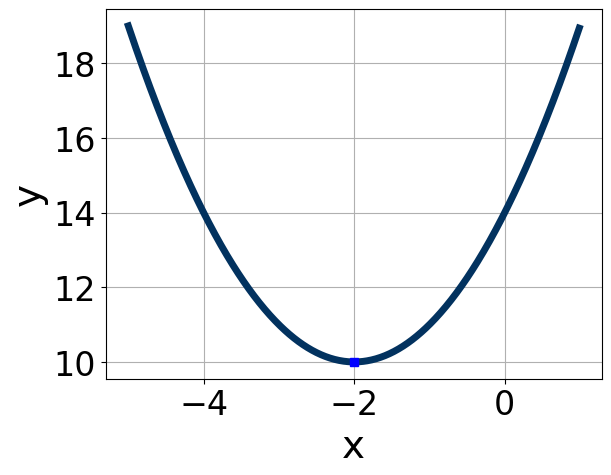
\includegraphics[width=0.5\textwidth]{../Figures/quadraticGraphToEquationCopyC.png}
\end{center}
\begin{enumerate}[label=\Alph*.]
\item \( a \in [-2.3, 0.2], \hspace*{5mm} b \in [2, 6], \text{ and } \hspace*{5mm} c \in [5, 8] \)
\item \( a \in [-0.4, 2.2], \hspace*{5mm} b \in [-5, -3], \text{ and } \hspace*{5mm} c \in [-8, -4] \)
\item \( a \in [-2.3, 0.2], \hspace*{5mm} b \in [-5, -3], \text{ and } \hspace*{5mm} c \in [5, 8] \)
\item \( a \in [-0.4, 2.2], \hspace*{5mm} b \in [-5, -3], \text{ and } \hspace*{5mm} c \in [12, 17] \)
\item \( a \in [-0.4, 2.2], \hspace*{5mm} b \in [2, 6], \text{ and } \hspace*{5mm} c \in [12, 17] \)

\end{enumerate} }
\litem{
Solve the quadratic equation below. Then, choose the intervals that the solutions belong to, with $x_1 \leq x_2$ (if they exist).\[ 16x^{2} -7 x -4 = 0 \]\begin{enumerate}[label=\Alph*.]
\item \( x_1 \in [-1.32, -0.5] \text{ and } x_2 \in [-0.1, 0.43] \)
\item \( x_1 \in [-5.76, -5.19] \text{ and } x_2 \in [11.79, 12.39] \)
\item \( x_1 \in [-0.34, 0.84] \text{ and } x_2 \in [0.41, 0.79] \)
\item \( x_1 \in [-17.37, -16.91] \text{ and } x_2 \in [17.43, 17.69] \)
\item \( \text{There are no Real solutions.} \)

\end{enumerate} }
\end{enumerate}

\end{document}